\documentclass[
	11pt,
]{beamer}

\graphicspath{{Images/}{./}}
\usetheme{Copenhagen}
\usefonttheme{default}
\useinnertheme{circles}
\usepackage{palatino}
\usepackage[default]{opensans}
\usepackage[english,russian]{babel}
\usepackage{booktabs}
\usepackage{graphicx}
\usepackage{caption}
\usepackage{subcaption}

\title[Генетический подход для частичных порядков]{Генетический выбор частичных порядков на множестве значений признаков в задаче классификации}
\author[Сорокин Олег, 317 группа ММП ВМК МГУ]{Сорокин Олег, 317}
\institute[ММП ВМК МГУ]{ММП ВМК МГУ}
\date[\today]{Спецсеминар \\ \today}

\begin{document}

\begin{frame}
	\titlepage
\end{frame}

\begin{frame}
	\tableofcontents
\end{frame}

\section{Постановки задач}

\subsection{Задача классификации по прецедентам}

\begin{frame}
	\frametitle{Задача классификации по прецедентам}
	
	Пусть задано некоторое множество объектов $M$, представимое в виде объединения $l$ непересекающихся множеств-классов $K_1, ..., K_l$. Элементы множества $M$ есть признаковые описания вида $x_1, ..., x_n$, где каждый из признаков принимает конечное число значений. Имеется $\{S_1, ..., S_m\} \subset M$ — множество объектов, принадлежность которых к определённым классам известна. Такие объекты называются прецедентами.
	
	\bigskip

	Требуется по предъявленному набору значений признаков $(b_1, ..., b_n) \in M$ определить класс объекта.

\end{frame}

\begin{frame}
	\frametitle{Частичные порядки в признаковых пространствах}
	
	Особый интерес представляют задачи со сложными отношениями на множествах значений признаков. Существуют эффективные подходы, основанные на независимом выборе линейных порядков.

\end{frame}

\subsection{Определения и обозначения}

\begin{frame}
	\frametitle{Определения и обозначения}
	
	\begin{block}{Определение}
		Элементы $x, y$ из частично упорядоченного множества $P$ называются сравнимыми, если $x$ предшествует $y$ (запись $x \leq y$).
	\end{block}

	\begin{block}{Определение}
		Пусть $P = P_1 \times ... \times P_n$, где $P_1, ..., P_n$ — конечные частично упорядоченные множества.

		Элемент $x = (x_1, ..., x_n) \in P$ следует за элементом $y = (y_1, ..., y_n) \in P$, если $x_i$ следует за $y_i$ ($i = 1, 2, ..., n$)
	\end{block}

\end{frame}

\begin{frame}
	\frametitle{Определения и обозначения}
	
	\begin{block}{Определение}
		Пусть $R \subset P$, $R^+$ — множество элементов, следующих за элементами из $R$. Элемент $x \in P \backslash R^+$ называется независимым от $R$ элементом множества $P$.

		\bigskip

		Если же кроме того $\forall y \in P \backslash R^+$ не выполнено отношение $x < y$, то $x$ — максимальный независимый от $R$ элемент множества $P$.
	\end{block}

\end{frame}

\subsection{Постановка задачи для произведения частичных порядков}

\begin{frame}
	
	Аналогично предыдущей постановке, пусть
	
	$M = \cup_{n=1}^{l}K_n$, где $K_i \cap K_j = \varnothing$ при $i \neq j$.

	\bigskip

	Пусть теперь $M$ представимо в виде $N_1 \times ... \times N_n$, где $N_i$ ($i \in \{1, 2, ..., n\}$) — конечное множество допустимых значений признака $x_i$. Не ограничивая общности, можно считать, что $N_i$ имеет наибольший элемент $k_i$.

	\bigskip

	Пусть также задан набор прецедентов $S_1 = (a_{11}, ..., a_{1n}), S_2 = (a_{21}, ..., a_{2n}), ..., S_m = (a_{m1}, ..., a_{mn})$.

	\bigskip

	Требуется по предъявленному набору значений признаков $(a_1, ..., a_n)$ объекта $S \in M$ (класс которого, вообще говоря, неизвестен) определить этот класс.
	
\end{frame}

\section{Упорядочение признаков и построение алгоритмов}

\subsection{Определения и обозначения}

\begin{frame}
	\frametitle{Определения и обозначения}
	
	\begin{block}{Определение}
		Пусть $R(K)$ и $R(\overline{K})$ — множества прецедентов из класса $K$ и не из класса $K$ соответственно.

		Будем говорить, что алгоритм $A$ классифицирует объект из $R(K)$ правильно, если $A$ относит его к классу $K$.
	\end{block}

	\begin{block}{Определение}
		Алгоритм $A$ называется корректным на $M$ алгоритмом, если $A$ правильно классифицирует каждый прецедент $S_1, ..., S_m$.
	\end{block}

\end{frame}

\begin{frame}
	\frametitle{Определения и обозначения}
	
	\begin{block}{Определение}
		Пусть $H = \{x_{j_1}, ..., x_{j_r}\}$, $\sigma = (\sigma_1, ..., \sigma_r)$, $\sigma_i \in N_{j_i}$ ($i = 1, 2, ..., r$). Пара $(\sigma, H)$ называется элементарным классификатором (эл. кл.) ранга $r$.
	\end{block}

	\begin{exampleblock}{Замечание}
		Эл. кл. порождает набор $S_{(\sigma, H)} = (\gamma_1, ..., \gamma_n)$, где $\gamma_{j_i} = \sigma_i$ ($i = 1, 2, ..., r$) и $\gamma_t = k_t$ при $t \notin \{j_1, ..., j_r\}$.
	\end{exampleblock}

	\begin{block}{Определение}
		$$
		\hat{B}(\sigma, S, H)=
		\begin{cases}
		1, a_{j_i} \leq \sigma_i (i=1, 2, ..., r) \\
		0, otherwise \\
		\end{cases}
		$$
	\end{block}

\end{frame}

\begin{frame}
	\frametitle{Определения и обозначения}
	
	\begin{block}{Определение}
		Эл. кл. $(\sigma, H)$ называется корректным для класса $K$, если нельзя указать пару объектов $S' \in R(K)$ и $S'' \in R(\overline{K})$: $\hat{B}(\sigma, S', H) = \hat{B}(\sigma, S'', H) = 1$.
	\end{block}

	\begin{block}{Определение}
		Корректный для класса $K$ эл. кл. $(\sigma, H)$ называется тупиковым, если $\forall (\sigma', H')$: $S_{(\sigma, H)} < S_{(\sigma', H')}$ не является корректным для класса $K$. 
	\end{block}
\end{frame}

\begin{frame}
	\frametitle{Определения и обозначения}

	\begin{block}{Определение}
		(Тупиковый) корректный эл. кл. называется (тупиковым) представительным для класса $K$, если хотя бы один прецедент из класса $K$ содержит данный эл. кл.
	\end{block}
\end{frame}

\subsection{Общая схема работы алгоритма}

\begin{frame}
	\frametitle{Общая схема работы алгоритма}

	\begin{enumerate}
		\item Обучение: для каждого класса $K$ строится некоторое множество представительных эл. кл. $C^A(K)$.
		\item Процедура голосования: вычисление оценок вида
			  $$\Gamma(S, K) = \frac{1}{|C^A(K)|} \sum_{(\sigma, H) \in C^A(K)} P_{(\sigma, H)} * \hat{B}(\sigma, S, H)$$
			  Здесь $P_{(\sigma, H)}$ — веса, обычно это число объектов из $R(K)$, содержащих $(\sigma, H)$.
	\end{enumerate}
\end{frame}

\subsection{Теоремы}

\begin{frame}
	\frametitle{Теоремы}
	
	\begin{block}{Теорема 1.}
		Алгоритм $A$ правильно классифицирует объект $S' \in R(K)$ тогда и только тогда, когда $S'$ — независимый от $R(\overline{K})$ элемент множества $M$.
	\end{block}

	\begin{block}{Теорема 2.}
		Пусть $\phi: M \rightarrow M \times M$ отображает объект $S = (a_1, ..., a_n)$ в объект $\phi(S) = (a_1, ..., a_n, a_{n+1}, ..., a_{2n}) \in M \times \tilde{M}$, где $\tilde{M}$ — множество с отношением порядка, обратным к отношению порядка в $M$.

		Если классы множества $M$ не пересекаются, то любой прецедент из класса $\phi(K)$ содержит представительный эл. кл. класса $\phi(K)$.
	\end{block}

\end{frame}

\subsection{Процедуры упорядочения признаков}

\begin{frame}
	\frametitle{Быстрая процедура независимого линейного упорядочения значений признаков}

	\begin{itemize}
		\item Пусть $\mu^{(1)}_{ij}(a)$ ($i \in \{1, 2, ..., l\}$, $j \in \{1,2 ..., \}$, $a \in N_j$) — доля прецедентов класса $K_i$, у которых признак $x_j$ принимает значение $a$. Аналогично определим $\mu^{(2)}_{ij}(a)$ для прецедентов не из класса $K$.
		\item Введём $\mu_{ij}(a) = \mu^{(1)}_{ij}(a) - \mu^{(2)}_{ij}(a)$ — вес значения $a$.
		\item $\forall y, z \in N_j$ считаем $y \leq z$ тогда и только тогда, когда $\mu_{ij}(y) \geq \mu_{ij}(z)$.
	\end{itemize}

	%\begin{exampleblock}{Замечание}
		%Пусть после задания порядка $S' \in R(K_i)$ классифицирован неправильно. По теореме 1 $\exists S'' \in R(\overline{K_i})$: $\mu_{ij}(a_j) \leq \mu_{ij}(b_j)$ (нетипичность описания $S'$).
	%\end{exampleblock}

	\begin{exampleblock}{Замечание}
		Порядок на множестве значений каждого признака выбирается независимо от выбора порядков для других признаков.
	\end{exampleblock}
\end{frame}

\begin{frame}
	\frametitle{Процедура корректного упорядочения значений признаков}

	\begin{itemize}
		\item Пусть для любого класса $K$ множество $C^A(K)$ содержит все тупиковые представительные эл. кл. класса $K$.
		\item Построим булеву матрицу $B_K$:
			\begin{enumerate}
				\item Каждой строке соответствует пара объектов $S' \in R(K)$, $S'' \in R(\overline{K})$, а каждому столбцу соответствует тройка $(j, a, b)$, где $j \in \{1, 2, ..., n\}$, $a, b \in N_j$, $a \neq b$.
				\item Элемент на пересечении строки $(S', S'')$ и столбца $(j, a, b)$ равен $1$, если признак $x_j$ равен $a$ и $b$ у объектов $S'$ и $S''$ соответственно.
			\end{enumerate}
	\end{itemize}
\end{frame}

\begin{frame}
	\frametitle{Процедура корректного упорядочения значений признаков}

	\begin{block}{Определение}
		Частичный порядок на $M$ называется $(A, K)$-корректным, если алгоритм $A$ правильно классифицирует каждый объект из $R(K)$.
	\end{block}

	\begin{block}{Теорема 3.}
		Частичный порядок, заданный на множестве $M$, является $(A, K)$-корректным тогда и только тогда, когда существует неприводимое покрытие $H$ матрицы $B_K$ такое, что $\forall j \in \{1, 2, ..., n\}$ и $\forall a, b \in N_j$ ($a < b$) столбец $(j, b, a)$ не входит в $H$.
	\end{block}
\end{frame}

\section{Генетический подход к поиску покрытий}

\subsection{Схема ГА, применение ГА к задаче о покрытии}

\begin{frame}
	\frametitle{Одна из схем генетического алгоритма}

	\begin{enumerate}
		\item Создаётся начальная популяция заданного объёма $N_p$. Для каждого индивида вычисляется приспособленность.
		\item Скрещивание. Из популяции выбираются два родителя. К ним применяется оператор скрещивания, получается потомок.
		\item Мутация. Потомок с заданной вероятностью подвергается мутации.
		\item Отбор. Вычисляется приспособленность потомка. Одна из менее приспособленных особей заменяется.
		\item Если не выполнено условие останова, то переход к п.2.
	\end{enumerate}
\end{frame}

\begin{frame}
	\frametitle{Одна из схем генетического алгоритма}

	Возможные способы представления особей:
	\begin{itemize}
		\item Бинарное. Хромосома есть бинарный вектор $g = (g_1, ..., g_n)$, где $g_i = 1$ тогда и только тогда, когда $i$-й столбец входит в набор столбцов $H$.
		\item Целочисленное. Хромосома есть целочисленный вектор $g = (g_1, ..., g_m)$, где $i$-я компонента равна номеру столбца, который покрывает строку с номером $i$.
	\end{itemize}
\end{frame}

\subsection{Формирование начальной популяции}

\begin{frame}
	\frametitle{Формирование начальной популяции}

	\begin{enumerate}
			\item
				\begin{itemize}
					\item В бинарном случае все компоненты выбираются случайно. Если полученный набор столбцов не является покрытием, то он дополняется новыми столбцами.
					\item Для целочисленного случая каждый раз случайно выбирается столбец из числа покрывающих нужную строку.
				\end{itemize}
			\item По вектору $g$ восстанавливается набор столбцов.
			\item Для каждого набора в порядке убывания весов столбцов проверяется, является ли $H \backslash \{j\}$ покрытием. Если да, то столбец исключается.
			\item Если в $P$ нет особи $(H, g)$, то она добавляется в $P$.
			\item Если сгенерировано достаточно особей, то процесс завершается. Иначе переход к п.1.
	\end{enumerate}
\end{frame}

\subsection{Скрещивание и мутация}

\begin{frame}
	\frametitle{Выбор родителей}

	\begin{itemize}
			\item Панмиксия — все особи имеют одинаковую вероятность.
			\item Инбридинг — первый случайно, второй наиболее похожий в каком-то смысле.
			\item Аутбридинг — первый случайно, второй наиболее отличный в каком-то смысле.
			\item Селективное скрещивание — устанавливается порог приспособленности для возможности скрещивания.
	\end{itemize}
\end{frame}

\begin{frame}
	\frametitle{Оператор скрещивания (кроссовер)}

	\begin{itemize}
			\item Одноточечный — в наборе хромосом происходит разрыв по случайной точке, а затем обмен получившимися частями.
			\item Многоточечный — выбираются несколько таких точек.
			\item Однородный — каждая хромосома копируется от одного из родителей случайным образом. Для бинарного случая
				  $$
				  g_i = 
				  \begin{cases}
					g^1_i, p_1 = \frac{f_2}{f_1 + f_2} \\
					g^2_i, p_2 = \frac{f_1}{f_1 + f_2} \\
				  \end{cases}
				  $$
	\end{itemize}
\end{frame}

\begin{frame}
	\frametitle{Мутация}

	В зависимости от модификации алгоритма, может зменяться одна или несколько случайно выбранных хромосом. При этом возможен выход из локального минимума.

	\bigskip

	Также можно изменять количество мутируемых хромосом со временем. Например,
	$$k(t) = k_0 * (1 - \frac{1}{C*t + 1})$$
\end{frame}

\begin{frame}
	\frametitle{Восстановление допустимости решения}

	При применении операторов скрещивания и мутации может возникнуть набор, не являющийся (неприводимым) покрытием. Пусть не покрыты строки $M_H$. В этом случае необходимо произвести процедуру восстановления допустимости решения:
	\begin{enumerate}
		\item $H$ дополняется до покрытия матрицы последовательным добавлением столбцов, покрывающих $M_H$ и минимизирующих $\frac{w_j}{|M_H \cap M_j|}$.
		\item Из $H$ конструируется неприводимое покрытие: убираем столбец $j$ (в порядке убывания весов), если $H \backslash \{j\}$ является покрытием. 
	\end{enumerate}
\end{frame}

\subsection{Селекция (функции приспособленности)}

\begin{frame}
	\frametitle{Функции приспособленности из статей (покрытие минимального веса)}
	\begin{enumerate}
		\item $f = \sum\limits_{i=1}^n[g_i = 1] * w_i$
		
		(в целочисленном случае аналогично, вычисляется вес покрытия).

		\item $f_i = w_i - \min\limits_{j \in \{1, ..., N\}} w_j + 1$
		
		(исправляет проблему предыдущей функции).
	\end{enumerate}
\end{frame}

\begin{frame}
	\frametitle{Функции приспособленности, которые можно попробовать для поиска любых покрытий}
	\begin{enumerate}
		\item Пусть $B'$ — матрица, составленная из столбцов $H$.
			  $f_1 = \sum\limits_{i=1}^m[\sum\limits_{j=1}^n B'_{ij} = 0] + 1$
		\item Некоторые строки покрываются малым числом столбцов. Если ГА их не включает, то застревает в локальном минимуме. Идея: за непокрытие таких строк "штрафовать" алгоритм.

			  Можно перейти ко взвешенной задаче и воспользоваться функцией
			  $$f_i = w_i - \min\limits_{j \in \{1, ..., N\}} w_j + 1$$
	\end{enumerate}
\end{frame}

\subsection{Программная реализация}

\begin{frame}
	\frametitle{Классический ГА для поиска минимальных покрытий}
	\begin{figure}
		\centering
		\begin{subfigure}{.5\textwidth}
		  \centering
		  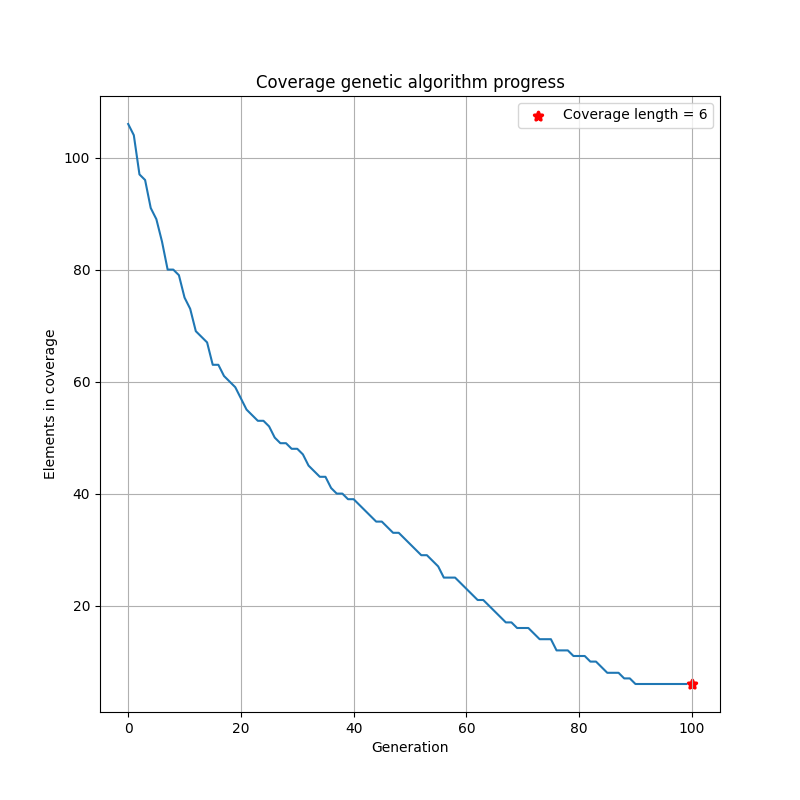
\includegraphics[width=1.\linewidth]{./images/Typical_progress_plot.png}
		  \label{fig:sub1}
		\end{subfigure}%
		\begin{subfigure}{.5\textwidth}
		  \centering
		  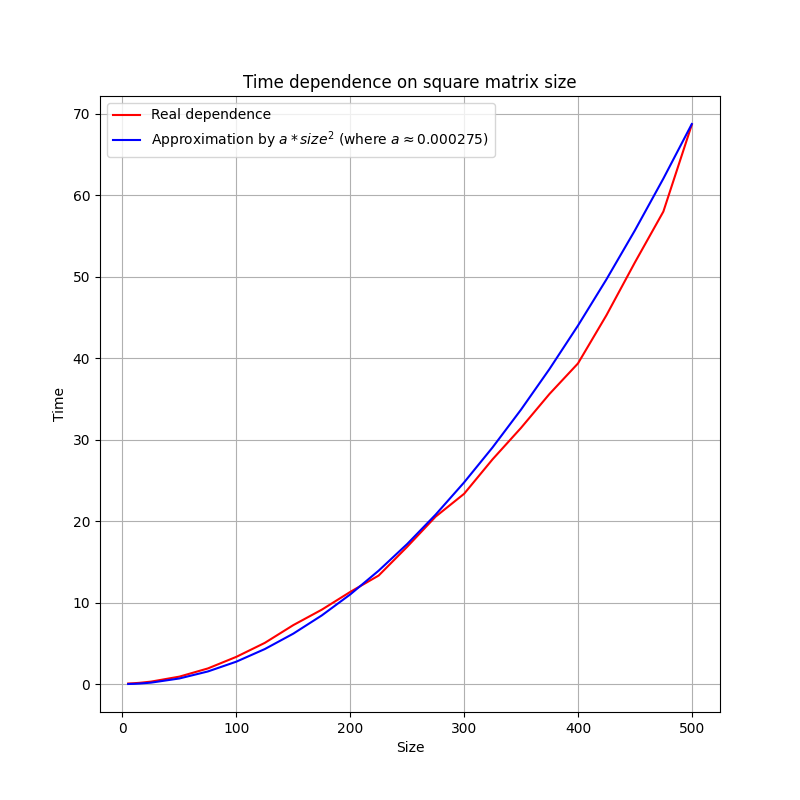
\includegraphics[width=1.\linewidth]{./images/Time_plot.png}
		  \label{fig:sub2}
		\end{subfigure}
		\label{fig:test}
		\end{figure}
\end{frame}

\end{document} 